\section{Il controllo attivo di un processo}

Il \textbf{controllo attivo di un processo} permette la gestione dei processi, macchine e impianti riducendo l'intervento umano.

I principi del controllo attivo si basano sull'azione diretta (\textbf{feedforward}) e sull'azione di retroazione (\textbf{feedback}).

Il controllo attivo elimina il problema di imporre un funzionamento desiderato ad un processo.

La variabile controllata del sistema deve essere uguale al segnale di riferimento(che noi desideriamo).

\subsection{Sistema}
Un \textbf{sistema} è un complesso in cui si distinguono grandezze variabili nel tempo.

Le funzioni che rappresentano l'andamento delle variabili nel tempo prendono il nome di \textbf{segnali}.


Il \textbf{modello matematico(m.m.)} di un sistema è la descrizone del sistema in termini matematici, permettendo di identificare ingressi, uscite e disturbi.


Un sistema è \textbf{statico} se l'uscita dipende esclusivamente dall'ingresso nello stesso instante $t$, senza considerare tutti gli istanti precedenti:
\begin{align}
	\exists \quad f: \mathbb{R} \rightarrow \mathbb{R} \ni y(t) = f(u(t)) \forall t \in \mathbb{R}
\end{align}


Mentre un sistema \textbf{dinamico} prende in considerazione tutti gli istanti precendenti $t$ nell'intervallo di tempo $(-\infty, t]$:

\begin{align}
	\exists \quad F: K \rightarrow J \ni y(t) = F(u(\cdot)|_{(-\infty, t]}) \forall t \in \mathbb{R}
\end{align}

I sistemi dinamici introducono un concetto di sistema in \textbf{quiete}, \textbf{condizioni asintotiche} e \textbf{a regime}.


Generalemnte si rappresentano tutte le possibili coppie causa effetto mediante l'utilizzo dei \textbf{behaviors($\mathbf{B}$)}:
\begin{align}
	\mathbf{B} = \{ (u(t), y(t)) : y(t) \text{ uscita per ingresso } u(t), \quad t \in (-\infty, +\infty)\}
\end{align}

Un sistema si dice \textbf{lineare} quando soddisfa la proprietà di \textbf{sovrapposizione degli effetti}:
\begin{align}
	 & \forall (u_1, y_1), (u_2, y_2) \in \mathbf{B},                                                                                                                            \\
	 & \forall \alpha_1, \alpha_2 \in \mathbb{R} \Rightarrow \alpha_1(u_1, y_1) + \alpha_2(u_2, y_2) = (\alpha_1 u_1 + \alpha_2 u_2, \alpha_1 y_1 + \alpha_2 y_2) \in \mathbf{B}
\end{align}

Introduco anche la \textbf{stazionarieà} come l'invarianza nel tempo, se applico un'ingresso ora o lo applico fra 1 giorno, avro la stessa uscita.

\subsection{Feedforward}
L'azione di comando dipende da:
\begin{itemize}
	\item obiettivo perseguito
	\item informazioni sul modello del sistema
	\item disturbi
\end{itemize}

\begin{figure}[!ht]
	\centering
	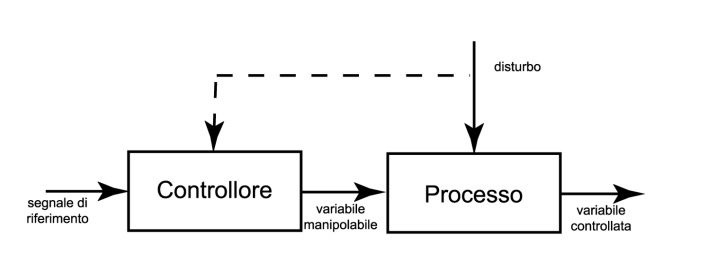
\includegraphics[width=0.5\textwidth]{./images/feedforward.png}
	\caption{Schema a blocchi di un sistema con feedforward}
	\label{fig:feedforward}
\end{figure}

\subsection{Feedback}

L'azione di comando dipende da:
\begin{itemize}
	\item obiettivo perseguito
	\item informazioni sul modello del sistema
	\item disturbi
	\item variabili controllate
\end{itemize}

\begin{figure}[!ht]
	\centering
	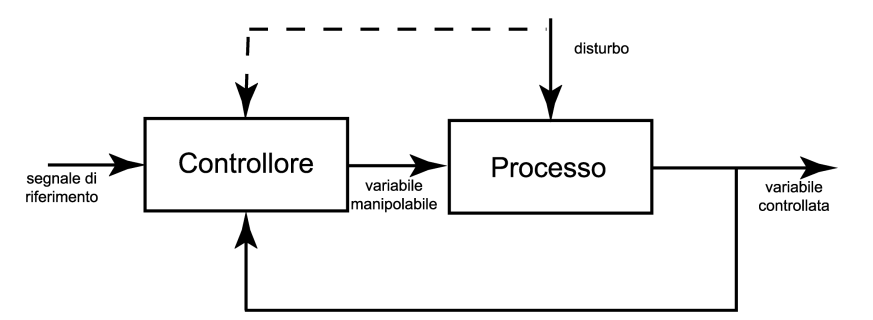
\includegraphics[width=0.5\textwidth]{./images/feedback.png}
	\caption{Schema a blocchi di un sistema con feedback}
	\label{fig:feedback}
\end{figure}


\subsection{Controllo diretto VS Controllo retroazionato}

L'errore in controllo diretto è $\pm 20 \%$ dove nel controllo in retroazione l'errore di inseguimento è circa $0.5\%$.

Il controllo in retroazione è efficace anche in presenza di perturbazioni sul processo. Parimenti, si potrebbe dimostrare che il controllo in retroazione è efficace anche in presenza di disturbi agenti sulla variabile controllata.


